% ---------------- CUSTOM MACROS ----------------
% Macro for Section Headers
% COLORS
\colorlet{protoncol}{red!68!black!80}
\colorlet{neutroncol}{green!68!black!80}
\colorlet{photoncol}{yellow!85!orange!95!black}
\colorlet{veccol}{green!50!black}
\colorlet{myred}{red!70!black}
\colorlet{mycontourred}{red!55!black!3} % for contour
\colorlet{mycontourred2}{red!55!black!6} % for contour
\colorlet{myblue}{blue!70!black}
\colorlet{mydarkred}{red!40!black}
\colorlet{mydarkblue}{blue!30!black}
\colorlet{CMScol}{red!80!black}
\colorlet{ATLAScol}{blue!80!black}

\tikzstyle{axis}=[->,thick,line cap=round]
\tikzstyle{detector}=[thick,draw=mydarkred,rotate around z=\ang]
\tikzstyle{beam pipe}=[draw=blue!20!black!50,fill=blue!20!black!10,rotate around z=\ang]
\tikzstyle{detector surface}=[red!60!black!10,opacity=0.5,rotate around z=\ang]



% STYLES
\tikzset{
	>=latex, % for LaTeX arrow head
	eta line/.style={->,black!60!red,thick,line cap=round},
	theta node/.style={black,pos=0.7,fill=white,scale=0.8,
		inner sep=1.5pt,rounded corners=3pt},
	mysmallarrow/.style={-{Latex[length=3,width=2.5]},draw=black,line width=0.6,
		angle radius=45,angle eccentricity=1.1},
	vector/.style={->,thick,green!60!black},
	photon/.style={->,line width=0.7,line cap=round,photoncol,decorate,decoration={
			snake,amplitude=.4mm,segment length=2.2mm,post length=1.5mm}
	},
	ball/.style={
		circle,draw=none,ball color=#1,postaction={
			fill=#1,fill opacity=0.8,draw=#1!40!black,line width=0.04}
	},
	ball/.default=protroncol,
	pics/nucleus/.style={%
		code={%
			\fill[protoncol] (0,0) circle(0.86*\R); % background to fill any holes
			\pgfmathsetmacro\Rball{0.18*\R} % ball radius
			\pgfmathsetmacro\Rcorr{\R-\Rball} % subtract ball radius
			\pgfmathsetmacro\C{min(1/(4*\Rcorr),0.24)} % put balls at edges closer in to create 3D ball effect
			\pgfmathsetmacro\D{1-4*\C*\Rcorr} % discriminant
			\pgfmathsetmacro\Rs{2*(\Rcorr)/(1+sqrt(\D)} % scaled total radius
			\message{^^J R=\R, R=\Rcorr, Rs=\Rs, C=\C, D=1-4cR=\D (must be >0)}
			\foreach \lay [evaluate={
				\r=\Rs*(\lay-0.05)/\Nlay; % ring radius
				\rC=\r-\C*\r*\r; % reduce outer radii to create 3D effect
				\aR=3*rand; % random angular offset
				\Nring=int(round(2*\rC*\N/(\Rs*(\Nlay+1)*(1-\C*\Rs*(2*\Nlay+1)/(3*\Nlay))))) % number of balls on this ring
			}] in {\Nlay,...,1}{
				\message{^^J N=\N, Nlay=\Nlay, Nring=\Nring, r=\r}
				\shufflelist{\Nring} % get shuffled list of sequence 1,...,\Nring
				\foreach \i [evaluate={
					\p=(rand+1)/2<0.39?1:0; % 0: neutron, 1: proton
					\is=int(\shuffledlist[\i]); % shuffled index
					\aB=\aR+360*(\is/\Nring)+2*rand/\Nring; % ball angle plus random offset
					\rB=\rC+0.04*rand % ball radius plus random radial offset
				}] in {1,...,\Nring}{
					%\message{^^J is=\is, i=\i, a=\aB, p=\p}
					\fill[ball=\ifodd\p protoncol\else neutroncol\fi]
					(\aB:\rB) circle(\Rball);
				}
			}
			\fill[ball=protoncol] (0,0) circle(\Rball);
			\foreach \ang in {0,60,90,120,180,-60,-90,-120}{
				\coordinate (-\ang) at (\ang:\R+1.3*\Rball);
			}
		}
	}
}
\def\shufflelist#1{ % get shuffled list of sequence 1,...,#1
	%\message{^^JShuffle list}
	\pgfmathsetmacro\tmplist{random(1,#1)} % first random item
	\readlist*\shuffledlist\tmplist % convert to array
	\newboolean{unique}
	\whiledo{\shuffledlistlen<#1}{ % try until list is of length = #1
		\pgfmathsetmacro\rx{random(1,#1)} % generate new random item
		\setboolean{unique}{true}
		\foreachitem \x \in \shuffledlist{ % loop over previous elements
			\ifnum \x=\rx % look if new number in list
			\setboolean{unique}{false} % already in list
			\breakforeach % stop looking and try again in next iteration
			\fi
		}
		\ifthenelse{\boolean{unique}}{ % found unique item !
			\xdef\tmplist{\tmplist,\rx} % add new unique item
			\readlist*\shuffledlist\tmplist % convert to array
		}{}
	}
}

\newcommand*{\vv}[1]{\vec{\mkern0mu#1}} % aligned vector arrow
\newcommand{\vhead}[1]{\textcolor[HTML]{B32222}{\sffamily\small\uppercase{#1}}}

% Macro for 3-point vertices 
% Args: #1=bottom-left style, #2=bottom-left label, #3=top-left style, #4=top-left label, #5=right style, #6=right label
\newcommand{\threevertex}[6]{%
	\begin{tikzpicture}[baseline=0, thick]
		\begin{feynman}
			\vertex [circle, fill=black, minimum size=3.5pt, inner sep=0pt] (v) at (0,0) {};
			\vertex (i1) at (240:1.5) {\(#2\)};
			\vertex (i2) at (120:1.5) {\(#4\)};
			\vertex [circle, fill=black, minimum size=2.5pt, inner sep=0pt] (o) at (1.5,0) {};
			\diagram* {
				(i1) -- [#1] (v) -- [#3] (i2),
				(v) -- [#5, edge label'=\(#6\)] (o)
			};
		\end{feynman}
	\end{tikzpicture}%
}

% Collider detector coordinate system
\newcommand{\detectorCoordinateSystem}{
\tdplotsetmaincoords{122.61461}{113.95680}
\begin{tikzpicture}[scale=2.8,tdplot_main_coords,rotate=76.53217]
	% VARIABLES
	\def\thetavec{60}
	\def\phivec{60}
	\def\L{3.1}     % detector length
	\def\R{0.75}    % detector cylinder radius
	\def\l{4.1}     % beam pipe length
	\def\r{0.04}    % beam pipe radius
	\def\rt{0.042}  % beam pipe radius + line thickness
	\def\xmax{1}    % maximum x axis
	\def\ymax{1.05} % maximum y axis
	\def\zmin{-\l/2-0.2} % minimum z axis
	\def\zmax{\l/2+0.3}  % maximum z axis
	\coordinate (O) at (0,0,0);
	\coordinate (Z) at (0,0,\L/2);
	\tdplotsetcoord{O''}{0.018}{90}{\phivec} % shifted origin for the pT arrow
	% |p| is chosen so the vector lands on the barrel surface: its transverse
	% projection (Pxy) then has radius exactly \R, so the beam-parallel line
	% through (Pxy) and (P) meets the +z endcap on its rim, at (Prim).
	\pgfmathsetmacro{\Rvec}{\R/sin(\thetavec)}
	\tdplotsetcoord{P}{\Rvec}{\thetavec}{\phivec}
	\coordinate (Prim) at ({\R*cos(\phivec)},{\R*sin(\phivec)},\L/2);
	
	% CYLINDER behind
	\def\ang{24} % rotate lines to simulate cylinder
	\fill[top color=red!50!black!4,bottom color=red!60!black!2,rotate around z=\ang]
	(0,\R,\L/2) --++ (0,0,-\L) arc(90:270:\R) --++ (0,0,\L) arc(270:90:\R) -- cycle;
	\fill[detector surface] % transverse plane at z=L/2
	(0,0,\L/2) --++ (0,\R,0) arc(90:270:\R) -- cycle;
	\fill[detector surface] % transverse plane at z=-L/2
	(0,0,-\L/2) --++ (0,\R,0) arc(90:270:\R) -- cycle;
	\tdplotdrawarc[detector,thin]{(0,0,\L/2)}{\R}{0}{360}{}{} % transverse plane at z=L/2
	\tdplotdrawarc[detector]{(0,0,-\L/2)}{\R}{0}{360}{}{} % transverse plane at z=-L/2
	\draw[detector,thin] % transverse plane at z=0
	(90:\R) arc (90:270:\R);
	\draw[detector,very thin] % transverse plane at z=0, top piece
	(90:\R) arc (90:90-\ang:\R);
	\draw[detector] (0,0,-\L/2)++(90:\R) --++ (0,0,\L); % top horizontal along z
	\draw[detector] (0,0,-\L/2)++(-90:\R) --++ (0,0,\L); % bottom horizontal along z
	
	% BEAM PIPE
	\tdplotdrawarc[beam pipe]{(0,0,-\l/2)}{\r}{0}{360}{}{}
	\draw[beam pipe] % beam pipe, thinner in middle
	(0,\r,-\l/2) -- (0,\r,-0.2*\l) -- (90:0.5*\r)
	-- (0,\r,0.2*\l) -- (0,\r,0.5*\l) arc(90:-90:\r)
	-- (0,-\r,0.2*\l) -- (-90:0.5*\r) --
	(0,-\r,-0.2*\l) -- (0,-\r,-\l/2) arc(-90:90:\r);
	\draw[beam pipe] (0,0,\l/2) circle(\r);
	
	% AXES
	\draw[axis] (0,0,0) -- (0,0,\zmax) node[above=2pt,right=1pt]{$z$}; % long
	\fill[CMScol] (O) circle(0.5pt) node[below=5pt] {IP};
	\draw[axis,-] (0,0,\zmin) -- (0,0,-0.020); % long
	\draw[axis] (0,0.019,0) -- (0,\ymax,0) node[above=1pt,right=1pt]{$y$};
	\draw[axis] (0.022,0,0) -- (\xmax,0,0) node[below=2pt,right=1pt]{$x$};
	
	% LABELS
	\node[mydarkred,above=1pt] at (0,\ymax,0) {$\eta=0$};
	\node[mydarkred,above=4pt,rotate around z=\ang] at (0,\R,0.30*\L) {$\eta>0$};
	\node[mydarkred,above=4pt,rotate around z=\ang] at (0,\R,-0.30*\L) {$\eta<0$};
	\node[mydarkred,left=1pt] at (0,0,\zmax) {$\eta=+\infty$};
	\node[mydarkred,right=1pt] at (0,0,\zmin) {$\eta=-\infty$};
	
	% CYLINDER front
	\draw[beam pipe,fill=none] (0,\r,-\l/2) arc(90:-90:\r);
	\fill[detector surface] % transverse plane at z=L/2
	(0,\rt,\L/2) --++ (0,\R-\rt,0) arc(90:-90:\R) --++ (0,\R-\rt,0) arc(-90:90:\rt);
	\fill[detector surface] % transverse plane at z=-L/2
	(0,\rt,-\L/2) --++ (0,\R-\rt,0) arc(90:-90:\R) --++ (0,\R-\rt,0) arc(-90:90:\rt);
	\tdplotdrawarc[detector]{(0,0,\L/2)}{\R}{-90}{90}{}{}
	\tdplotdrawarc[detector]{(0,0,-\L/2)}{\R}{-90}{90}{}{}
	\draw[beam pipe,fill=none] (0,\r,\l/2) arc(90:-90:\r);
	\draw[detector,very thin] % transverse plane at z=0, front piece
	(90-\ang:\R) arc (90-\ang:-90:\R);
	
	% VECTORS
	\draw[dashed,myred] (Pz) -- (P);
	\draw[dashed,myred,line join=round] (Py) -- (Pxy) -- (P) -- (Prim);
	\draw[dashed,myred] (Z) -- (Prim); % endcap radius at azimuth \phivec
	\draw[->,red,line cap=round] (O'') -- (Pxy) node[below=1pt,right=1pt] {$\vv{p}_\mathrm{T}$};
	\draw[->,red] (O) -- (P) node[above=1pt,left=1pt] {$\vv{p}$};
	
	% ANGLES
	% Each angle is drawn twice: once as the arc itself (no label), then as a
	% label-only pass with "draw=none" at a larger radius, so the label sits
	% radially outside the arc -- on the far side from the arc's centre.
	\def\labelgap{0.16} % radial offset of an angle label beyond its arc
	\tdplotdrawarc[thick,mycontourred]{(O)}{0.22}{4}{0.7*\phivec}{}{} % contour
	\tdplotdrawarc[->]{(O)}{0.22}{0}{\phivec}{}{}
	\tdplotdrawarc[draw=none]{(O)}{0.22+\labelgap}{0}{\phivec}
	{}{\contour{mycontourred}{$\varphi$}}
	\tdplotdrawarc[->,rotate around z=\phivec-90,rotate around y=-90]
	{(O)}{0.42}{0}{\thetavec}{}{}
	\tdplotdrawarc[draw=none,rotate around z=\phivec-90,rotate around y=-90]
	{(O)}{0.42+\labelgap}{0}{\thetavec}{}{$\theta$}
	\tdplotdrawarc[-{>[bend=1]},rotate around z=\phivec-90,rotate around y=-90,line cap=round]
	{(O)}{0.34}{90}{\thetavec}{}{}
	\tdplotdrawarc[draw=none,rotate around z=\phivec-90,rotate around y=-90]
	{(O)}{0.34+\labelgap}{90}{\thetavec}{}{$\eta$}
	\draw[mydarkred,line cap=round] (0.004,0,\L/2) --++ (\R,0,0); % phi reference at z=L/2
	\tdplotdrawarc[thick,mycontourred2]{(Z)}{0.22}{4}{0.7*\phivec}{}{} % contour
	\tdplotdrawarc[->]{(Z)}{0.22}{0}{\phivec}{}{}
	\tdplotdrawarc[draw=none]{(Z)}{0.22+\labelgap}{0}{\phivec}
	{}{\contour{mycontourred2}{$\varphi$}}
	
\end{tikzpicture}
}

% Macro for a propagator (2-point function)
% Args: #1=edge style, #2=left label, #3=right label, #4=momentum label
\newcommand{\propagator}[4]{%
	\begin{tikzpicture}[baseline=0, thick]
		\begin{feynman}
			\vertex (l) at (-1.1,0) {\(#2\)};
			\vertex (r) at ( 1.1,0) {\(#3\)};
			\diagram* { (l) -- [#1, edge label=\(#4\)] (r) };
		\end{feynman}
	\end{tikzpicture}%
}

% Macro for a Y-shaped 3-point vertex: one leg up, two legs down.
% The two lower legs are drawn as a single line THROUGH the vertex, so that
% fermion/ghost arrows follow the flow (down-left in, down-right out).
% Args, per leg: style / end label / momentum label (empty momentum = no label)
%   #1 #2 #3 = up leg,  #4 #5 #6 = lower-left leg,  #7 #8 #9 = lower-right leg
\newcommand{\yvertex}[9]{%
	\begin{tikzpicture}[baseline=0, thick]
		\begin{feynman}
			\vertex [circle, fill=black, minimum size=3.5pt, inner sep=0pt] (v) at (0,0) {};
			\vertex (u) at (90:1.5) {\(#2\)};
			\vertex (dl) at (215:1.5) {\(#5\)};
			\vertex (dr) at (325:1.5) {\(#8\)};
			\diagram* {
				(dl) -- [#4] (v) -- [#7] (dr),
				(v) -- [#1] (u),
			};
		\end{feynman}
		% momentum labels, placed by hand so the two lower ones stay apart
		\node[anchor=east] at ([xshift=-2pt]90:0.85) {\(#3\)};
		\node[anchor=south] at ([yshift=3pt]215:0.80) {\(#6\)};
		\node[anchor=south] at ([yshift=3pt]325:0.80) {\(#9\)};
	\end{tikzpicture}%
}

% Collinear factorization of a hadron-hadron hard scattering:
% the two incoming hadrons (double lines) each supply a parton carrying a
% fraction x of the hadron momentum, drawn from the parton distributions
% f_i(x_1), f_j(x_2); the partons enter the hard cross section
% sigma-hat_ij(alpha_s), and the beam remnants / outgoing partons leave as
% three-line legs.  Takes no arguments; use inside a figure.
\newcommand{\factorizationdiagram}{%
	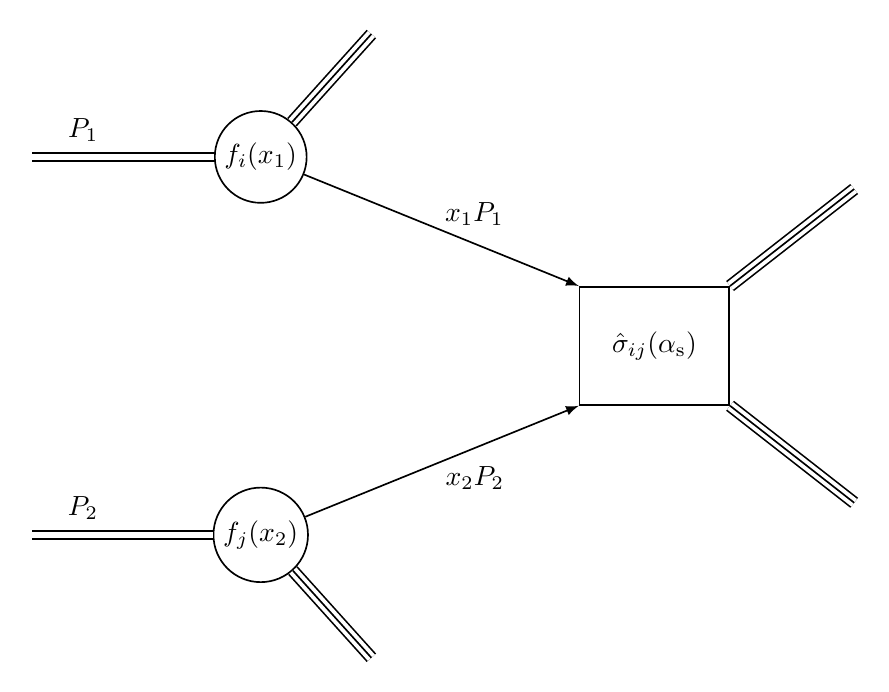
\begin{tikzpicture}[
			>=latex, line width=0.6pt,
			hadron/.style={double,double distance=2.2pt}, % incoming hadron: two lines
			triple/.style={double,double distance=3.4pt}, % outer pair of a three-line leg
		]
		% --- parton distributions and the hard-scattering blob
		\node[draw,circle,inner sep=2pt] (p1) at (0, 2.4) {$f_i(x_1)$};
		\node[draw,circle,inner sep=2pt] (p2) at (0,-2.4) {$f_j(x_2)$};
		\node[draw,minimum width=1.9cm,minimum height=1.5cm,inner sep=2pt]
		(sig) at (5.0,0) {$\hat{\sigma}_{ij}(\alpha_{\rm s})$};

		% --- endpoints of the beam remnants and the outgoing partons
		\path (p1) ++(48:2.1) coordinate (rem1);
		\path (p2) ++(-48:2.1) coordinate (rem2);
		\path (sig.north east) ++(38:2.0) coordinate (out1);
		\path (sig.south east) ++(-38:2.0) coordinate (out2);

		% --- incoming hadrons
		\draw[hadron] (-2.9, 2.4) -- (p1) node[pos=0.28,above=2pt] {$P_1$};
		\draw[hadron] (-2.9,-2.4) -- (p2) node[pos=0.28,above=2pt] {$P_2$};

		% --- three-line legs: beam remnants and outgoing partons
		\foreach \s/\e in {p1/rem1, p2/rem2, sig.north east/out1, sig.south east/out2}{
				\draw[triple] (\s) -- (\e);
				\draw (\s) -- (\e); % middle line
			}

		% --- the two partons entering the hard scattering
		\draw[->] (p1) -- (sig.north west) node[pos=0.62,above=3pt] {$x_1P_1$};
		\draw[->] (p2) -- (sig.south west) node[pos=0.62,below=3pt] {$x_2P_2$};
	\end{tikzpicture}%
}

% ---------------------------------------------------------------------------
% Leading-order 2 -> 2 partonic diagrams for jet production (tab:jetdiagrams).
% Incoming partons enter from the left, outgoing partons leave to the right.
% \jetdiagw and \jetdiagh are the half-width and half-height of every diagram,
% so the whole set is drawn on one common scale; change them to rescale the
% entire table at once.  Naming: trailing T/U/S = t-, u-, s-channel,
% X = the four-gluon contact term.
% ---------------------------------------------------------------------------
\def\jetdiagw{1.00} % half-width  of a 2->2 diagram
\def\jetdiagh{0.48} % half-height of a 2->2 diagram

% t-channel gluon exchange between two quark lines.
% Args: #1 = lower-line flavour label, #2 = upper-line flavour label.
% Used for both q q' -> q q' (distinct labels) and q q -> q q (same label).
\newcommand{\diagqqpT}[2]{%
	\begin{tikzpicture}[baseline=0, thick]
		\begin{feynman}
			\vertex (v1) at (0,-\jetdiagh);
			\vertex (v2) at (0, \jetdiagh);
			\vertex (i1) at (-\jetdiagw,-\jetdiagh) {\(#1\)};
			\vertex (o1) at ( \jetdiagw,-\jetdiagh) {\(#1\)};
			\vertex (i2) at (-\jetdiagw, \jetdiagh) {\(#2\)};
			\vertex (o2) at ( \jetdiagw, \jetdiagh) {\(#2\)};
			\diagram* {
				(i1) -- [fermion] (v1) -- [fermion] (o1),
				(i2) -- [fermion] (v2) -- [fermion] (o2),
				(v1) -- [gluon] (v2),
			};
		\end{feynman}
	\end{tikzpicture}%
}

% u-channel partner of the above: identical quarks, so the two outgoing legs
% are interchanged and the final-state lines cross.  Arg: #1 = flavour label.
\newcommand{\diagqqU}[1]{%
	\begin{tikzpicture}[baseline=0, thick]
		\begin{feynman}
			\vertex (v1) at (-0.35,-\jetdiagh);
			\vertex (v2) at (-0.35, \jetdiagh);
			\vertex (i1) at (-\jetdiagw,-\jetdiagh) {\(#1\)};
			\vertex (i2) at (-\jetdiagw, \jetdiagh) {\(#1\)};
			\vertex (o1) at ( \jetdiagw, \jetdiagh) {\(#1\)};
			\vertex (o2) at ( \jetdiagw,-\jetdiagh) {\(#1\)};
			\diagram* {
				(i1) -- [fermion] (v1) -- [fermion] (o1),
				(i2) -- [fermion] (v2) -- [fermion] (o2),
				(v1) -- [gluon] (v2),
			};
		\end{feynman}
	\end{tikzpicture}%
}

% t-channel gluon exchange between a quark line (top, left to right) and an
% antiquark line (bottom, right to left).
% Args: #1 = quark flavour, #2 = antiquark flavour (bar is supplied here).
% Covers q qbar' -> q qbar' and the t-channel of q qbar -> q qbar.
\newcommand{\diagqqbpT}[2]{%
	\begin{tikzpicture}[baseline=0, thick]
		\begin{feynman}
			\vertex (v1) at (0,-\jetdiagh);
			\vertex (v2) at (0, \jetdiagh);
			\vertex (i1) at (-\jetdiagw,-\jetdiagh) {\(\bar{#2}\)};
			\vertex (o1) at ( \jetdiagw,-\jetdiagh) {\(\bar{#2}\)};
			\vertex (i2) at (-\jetdiagw, \jetdiagh) {\(#1\)};
			\vertex (o2) at ( \jetdiagw, \jetdiagh) {\(#1\)};
			\diagram* {
				(o1) -- [fermion] (v1) -- [fermion] (i1),
				(i2) -- [fermion] (v2) -- [fermion] (o2),
				(v1) -- [gluon] (v2),
			};
		\end{feynman}
	\end{tikzpicture}%
}

% s-channel quark-antiquark annihilation through a single gluon into a
% quark-antiquark pair.  Args: #1 = incoming flavour, #2 = outgoing flavour.
% Covers q qbar -> q' qbar' and the s-channel of q qbar -> q qbar.
\newcommand{\diagqqbAnn}[2]{%
	\begin{tikzpicture}[baseline=0, thick]
		\begin{feynman}
			\vertex (i1) at (-\jetdiagw, \jetdiagh) {\(#1\)};
			\vertex (i2) at (-\jetdiagw,-\jetdiagh) {\(\bar{#1}\)};
			\vertex (v1) at (-0.35,0);
			\vertex (v2) at ( 0.35,0);
			\vertex (o1) at ( \jetdiagw, \jetdiagh) {\(#2\)};
			\vertex (o2) at ( \jetdiagw,-\jetdiagh) {\(\bar{#2}\)};
			\diagram* {
				(i1) -- [fermion] (v1) -- [fermion] (i2),
				(v1) -- [gluon] (v2),
				(o2) -- [fermion] (v2) -- [fermion] (o1),
			};
		\end{feynman}
	\end{tikzpicture}%
}

% g g -> q qbar, s-channel through the three-gluon vertex.
\newcommand{\diagggqqS}{%
	\begin{tikzpicture}[baseline=0, thick]
		\begin{feynman}
			\vertex (i1) at (-\jetdiagw, \jetdiagh) {\(g\)};
			\vertex (i2) at (-\jetdiagw,-\jetdiagh) {\(g\)};
			\vertex (v1) at (-0.35,0);
			\vertex (v2) at ( 0.35,0);
			\vertex (o1) at ( \jetdiagw, \jetdiagh) {\(q\)};
			\vertex (o2) at ( \jetdiagw,-\jetdiagh) {\(\bar{q}\)};
			\diagram* {
				(i1) -- [gluon] (v1),
				(i2) -- [gluon] (v1),
				(v1) -- [gluon] (v2),
				(o2) -- [fermion] (v2) -- [fermion] (o1),
			};
		\end{feynman}
	\end{tikzpicture}%
}

% g g -> q qbar, t-channel quark exchange.
\newcommand{\diagggqqT}{%
	\begin{tikzpicture}[baseline=0, thick]
		\begin{feynman}
			\vertex (i1) at (-\jetdiagw, \jetdiagh) {\(g\)};
			\vertex (i2) at (-\jetdiagw,-\jetdiagh) {\(g\)};
			\vertex (v1) at (0, \jetdiagh);
			\vertex (v2) at (0,-\jetdiagh);
			\vertex (o1) at ( \jetdiagw, \jetdiagh) {\(q\)};
			\vertex (o2) at ( \jetdiagw,-\jetdiagh) {\(\bar{q}\)};
			\diagram* {
				(i1) -- [gluon] (v1),
				(i2) -- [gluon] (v2),
				(o2) -- [fermion] (v2),
				(v2) -- [fermion] (v1),
				(v1) -- [fermion] (o1),
			};
		\end{feynman}
	\end{tikzpicture}%
}

% g g -> q qbar, u-channel: the outgoing quark and antiquark are interchanged.
\newcommand{\diagggqqU}{%
	\begin{tikzpicture}[baseline=0, thick]
		\begin{feynman}
			\vertex (i1) at (-\jetdiagw, \jetdiagh) {\(g\)};
			\vertex (i2) at (-\jetdiagw,-\jetdiagh) {\(g\)};
			\vertex (v1) at (-0.30, \jetdiagh);
			\vertex (v2) at (-0.30,-\jetdiagh);
			\vertex (o1) at ( \jetdiagw, \jetdiagh) {\(q\)};
			\vertex (o2) at ( \jetdiagw,-\jetdiagh) {\(\bar{q}\)};
			\diagram* {
				(i1) -- [gluon] (v1),
				(i2) -- [gluon] (v2),
				(o2) -- [fermion] (v1),
				(v1) -- [fermion] (v2),
				(v2) -- [fermion] (o1),
			};
		\end{feynman}
	\end{tikzpicture}%
}

% q g -> q g, s-channel quark exchange.
\newcommand{\diagqgS}{%
	\begin{tikzpicture}[baseline=0, thick]
		\begin{feynman}
			\vertex (i1) at (-\jetdiagw, \jetdiagh) {\(q\)};
			\vertex (i2) at (-\jetdiagw,-\jetdiagh) {\(g\)};
			\vertex (v1) at (-0.35,0);
			\vertex (v2) at ( 0.35,0);
			\vertex (o1) at ( \jetdiagw, \jetdiagh) {\(q\)};
			\vertex (o2) at ( \jetdiagw,-\jetdiagh) {\(g\)};
			\diagram* {
				(i1) -- [fermion] (v1),
				(i2) -- [gluon] (v1),
				(v1) -- [fermion] (v2),
				(v2) -- [fermion] (o1),
				(v2) -- [gluon] (o2),
			};
		\end{feynman}
	\end{tikzpicture}%
}

% q g -> q g, t-channel gluon exchange.
\newcommand{\diagqgT}{%
	\begin{tikzpicture}[baseline=0, thick]
		\begin{feynman}
			\vertex (v1) at (0, \jetdiagh);
			\vertex (v2) at (0,-\jetdiagh);
			\vertex (i1) at (-\jetdiagw, \jetdiagh) {\(q\)};
			\vertex (o1) at ( \jetdiagw, \jetdiagh) {\(q\)};
			\vertex (i2) at (-\jetdiagw,-\jetdiagh) {\(g\)};
			\vertex (o2) at ( \jetdiagw,-\jetdiagh) {\(g\)};
			\diagram* {
				(i1) -- [fermion] (v1) -- [fermion] (o1),
				(i2) -- [gluon] (v2) -- [gluon] (o2),
				(v1) -- [gluon] (v2),
			};
		\end{feynman}
	\end{tikzpicture}%
}

% q g -> q g, u-channel quark exchange: the outgoing quark and gluon are
% interchanged relative to the t-channel diagram.
\newcommand{\diagqgU}{%
	\begin{tikzpicture}[baseline=0, thick]
		\begin{feynman}
			\vertex (v1) at (0, \jetdiagh);
			\vertex (v2) at (0,-\jetdiagh);
			\vertex (i1) at (-\jetdiagw, \jetdiagh) {\(q\)};
			\vertex (o1) at ( \jetdiagw, \jetdiagh) {\(g\)};
			\vertex (i2) at (-\jetdiagw,-\jetdiagh) {\(g\)};
			\vertex (o2) at ( \jetdiagw,-\jetdiagh) {\(q\)};
			\diagram* {
				(i1) -- [fermion] (v1),
				(v1) -- [gluon] (o1),
				(i2) -- [gluon] (v2),
				(v1) -- [fermion] (v2),
				(v2) -- [fermion] (o2),
			};
		\end{feynman}
	\end{tikzpicture}%
}

% q qbar -> g g, s-channel annihilation through the three-gluon vertex.
\newcommand{\diagqqbS}{%
	\begin{tikzpicture}[baseline=0, thick]
		\begin{feynman}
			\vertex (i1) at (-\jetdiagw, \jetdiagh) {\(q\)};
			\vertex (i2) at (-\jetdiagw,-\jetdiagh) {\(\bar{q}\)};
			\vertex (v1) at (-0.35,0);
			\vertex (v2) at ( 0.35,0);
			\vertex (o1) at ( \jetdiagw, \jetdiagh) {\(g\)};
			\vertex (o2) at ( \jetdiagw,-\jetdiagh) {\(g\)};
			\diagram* {
				(i1) -- [fermion] (v1) -- [fermion] (i2),
				(v1) -- [gluon] (v2),
				(v2) -- [gluon] (o1),
				(v2) -- [gluon] (o2),
			};
		\end{feynman}
	\end{tikzpicture}%
}

% q qbar -> g g, t-channel quark exchange.
\newcommand{\diagqqbT}{%
	\begin{tikzpicture}[baseline=0, thick]
		\begin{feynman}
			\vertex (i1) at (-\jetdiagw, \jetdiagh) {\(q\)};
			\vertex (i2) at (-\jetdiagw,-\jetdiagh) {\(\bar{q}\)};
			\vertex (v1) at (0, \jetdiagh);
			\vertex (v2) at (0,-\jetdiagh);
			\vertex (o1) at ( \jetdiagw, \jetdiagh) {\(g\)};
			\vertex (o2) at ( \jetdiagw,-\jetdiagh) {\(g\)};
			\diagram* {
				(i1) -- [fermion] (v1),
				(v1) -- [fermion] (v2),
				(v2) -- [fermion] (i2),
				(v1) -- [gluon] (o1),
				(v2) -- [gluon] (o2),
			};
		\end{feynman}
	\end{tikzpicture}%
}

% q qbar -> g g, u-channel: as above with the two outgoing gluons interchanged.
\newcommand{\diagqqbU}{%
	\begin{tikzpicture}[baseline=0, thick]
		\begin{feynman}
			\vertex (i1) at (-\jetdiagw, \jetdiagh) {\(q\)};
			\vertex (i2) at (-\jetdiagw,-\jetdiagh) {\(\bar{q}\)};
			\vertex (v1) at (-0.30, \jetdiagh);
			\vertex (v2) at (-0.30,-\jetdiagh);
			\vertex (o1) at ( \jetdiagw, \jetdiagh) {\(g\)};
			\vertex (o2) at ( \jetdiagw,-\jetdiagh) {\(g\)};
			\diagram* {
				(i1) -- [fermion] (v1),
				(v1) -- [fermion] (v2),
				(v2) -- [fermion] (i2),
				(v1) -- [gluon] (o2),
				(v2) -- [gluon] (o1),
			};
		\end{feynman}
	\end{tikzpicture}%
}

% g g -> g g, s-channel through two three-gluon vertices.
\newcommand{\diagggS}{%
	\begin{tikzpicture}[baseline=0, thick]
		\begin{feynman}
			\vertex (i1) at (-\jetdiagw, \jetdiagh) {\(g\)};
			\vertex (i2) at (-\jetdiagw,-\jetdiagh) {\(g\)};
			\vertex (v1) at (-0.35,0);
			\vertex (v2) at ( 0.35,0);
			\vertex (o1) at ( \jetdiagw, \jetdiagh) {\(g\)};
			\vertex (o2) at ( \jetdiagw,-\jetdiagh) {\(g\)};
			\diagram* {
				(i1) -- [gluon] (v1),
				(i2) -- [gluon] (v1),
				(v1) -- [gluon] (v2),
				(v2) -- [gluon] (o1),
				(v2) -- [gluon] (o2),
			};
		\end{feynman}
	\end{tikzpicture}%
}

% g g -> g g, t-channel gluon exchange.
\newcommand{\diagggT}{%
	\begin{tikzpicture}[baseline=0, thick]
		\begin{feynman}
			\vertex (v1) at (0, \jetdiagh);
			\vertex (v2) at (0,-\jetdiagh);
			\vertex (i1) at (-\jetdiagw, \jetdiagh) {\(g\)};
			\vertex (o1) at ( \jetdiagw, \jetdiagh) {\(g\)};
			\vertex (i2) at (-\jetdiagw,-\jetdiagh) {\(g\)};
			\vertex (o2) at ( \jetdiagw,-\jetdiagh) {\(g\)};
			\diagram* {
				(i1) -- [gluon] (v1) -- [gluon] (o1),
				(i2) -- [gluon] (v2) -- [gluon] (o2),
				(v1) -- [gluon] (v2),
			};
		\end{feynman}
	\end{tikzpicture}%
}

% g g -> g g, u-channel: the two outgoing gluons are interchanged.
\newcommand{\diagggU}{%
	\begin{tikzpicture}[baseline=0, thick]
		\begin{feynman}
			\vertex (v1) at (-0.30, \jetdiagh);
			\vertex (v2) at (-0.30,-\jetdiagh);
			\vertex (i1) at (-\jetdiagw, \jetdiagh) {\(g\)};
			\vertex (o1) at ( \jetdiagw, \jetdiagh) {\(g\)};
			\vertex (i2) at (-\jetdiagw,-\jetdiagh) {\(g\)};
			\vertex (o2) at ( \jetdiagw,-\jetdiagh) {\(g\)};
			\diagram* {
				(i1) -- [gluon] (v1),
				(v1) -- [gluon] (o2),
				(i2) -- [gluon] (v2),
				(v2) -- [gluon] (o1),
				(v1) -- [gluon] (v2),
			};
		\end{feynman}
	\end{tikzpicture}%
}

% g g -> g g, the four-gluon contact term (cf. the four-gluon vertex of
% tab:qcdrules), redrawn here on the common 2->2 scale.
\newcommand{\diagggX}{%
	\begin{tikzpicture}[baseline=0, thick]
		\begin{feynman}
			\vertex (v) at (0,0);
			\vertex (i1) at (-\jetdiagw, \jetdiagh) {\(g\)};
			\vertex (i2) at (-\jetdiagw,-\jetdiagh) {\(g\)};
			\vertex (o1) at ( \jetdiagw, \jetdiagh) {\(g\)};
			\vertex (o2) at ( \jetdiagw,-\jetdiagh) {\(g\)};
			\diagram* {
				(i1) -- [gluon] (v),
				(i2) -- [gluon] (v),
				(v) -- [gluon] (o1),
				(v) -- [gluon] (o2),
			};
		\end{feynman}
	\end{tikzpicture}%
}

% Macro for 4-point vertices
% Args: #1=top-left style, #2=top-left label, #3=bottom-left style, #4=bottom-left label,
%       #5=top-right style, #6=top-right label, #7=bottom-right style, #8=bottom-right label
\newcommand{\fourvertex}[8]{%
	\begin{tikzpicture}[baseline=0, thick]
		\begin{feynman}
			\vertex [circle, fill=black, minimum size=3.5pt, inner sep=0pt] (v) at (0,0) {};
			\vertex (i1) at (135:1.5) {\(#2\)};
			\vertex (i2) at (225:1.5) {\(#4\)};
			\vertex (o1) at (45:1.5) {\(#6\)};
			\vertex (o2) at (-45:1.5) {\(#8\)};
			\diagram* {
				(i1) -- [#1] (v),
				(i2) -- [#3] (v),
				(v) -- [#5] (o1),
				(v) -- [#7] (o2),
			};
		\end{feynman}
	\end{tikzpicture}%
}